% multiple1902 <multiple1902@gmail.com>
% intro.tex
% Copyright 2011~2012, multiple1902 (Weisi Dai)
% https://code.google.com/p/xjtuthesis/
%
% It is strongly recommended that you read documentations located at
%   http://code.google.com/p/xjtuthesis/wiki/Landing?tm=6
% in advance of your compilation if you have not read them before.
%
% This work may be distributed and/or modified under the
% conditions of the LaTeX Project Public License, either version 1.3
% of this license or (at your option) any later version.
% The latest version of this license is in
%   http://www.latex-project.org/lppl.txt
% and version 1.3 or later is part of all distributions of LaTeX
% version 2005/12/01 or later.
%
% This work has the LPPL maintenance status `maintained'.
%
% The Current Maintainer of this work is Weisi Dai.
%

\chapter{绪论}
\echapter{Introduction}

本章主要对本文研究内容的背景和意义进行介绍,以及对国内外研究在此领域的现状进行讨论,并给出本文的主要研究内容和组织结构。

    \section{背景}
    \esection{Background}

    文字是用来存储信息或记录语言的图像符号,图像中的文字是可以直接传递内容语义的重要信息源,而让计算机能够定位并理解数字图像中的文字,即文字检测和识别,直到现在仍是图像处理与模式识别领域中的研究热点。其对于图像检索,盲人辅助系统,无人驾驶导航及文档图像处理等人工智能系统均起到巨大的辅助作用,如图\ref{fig.c1_apply}所示:
    
    \begin{figure*}[!h]
    \centering
    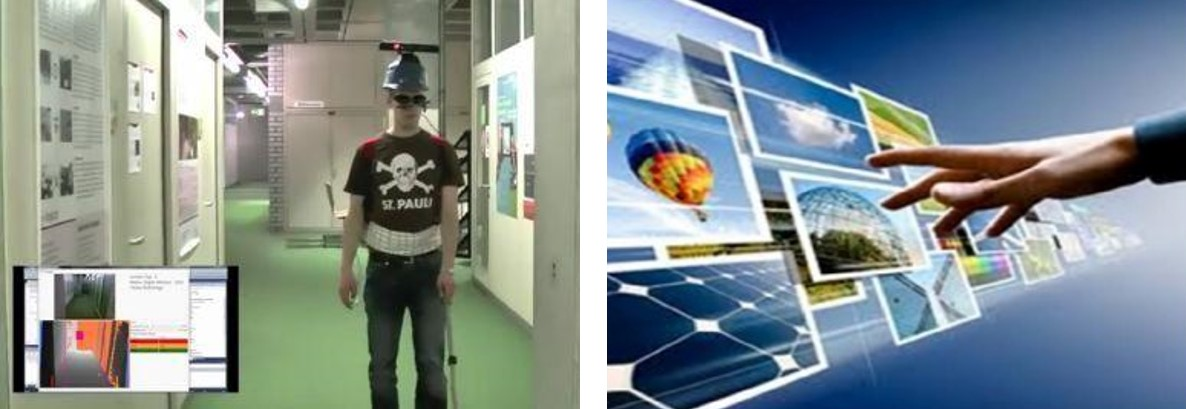
\includegraphics[width=\textwidth]{./figures/c1_apply_1.jpg}
    \begin{minipage}[t]{0.48\linewidth}
    \centerline{ \small (a) 盲人辅助设备}
    \end{minipage}
    \begin{minipage}[t]{0.48\linewidth}
    \centerline{ \small (b) 基于内容的海量图像检索}
    \end{minipage}
    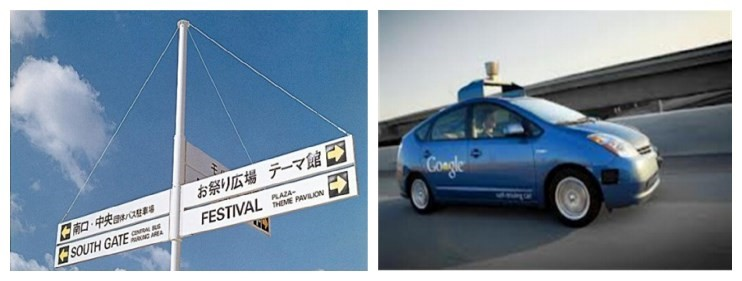
\includegraphics[width=\textwidth]{./figures/c1_apply_2.jpg}
    \begin{minipage}[t]{0.48\linewidth}
    \centerline{ \small (d) 国外旅游辅助}
    \end{minipage}
    \begin{minipage}[t]{0.48\linewidth}
    \centerline{ \small (e) 无人驾驶导航系统}
    \end{minipage}
    \caption{自然场景中文字检测与识别的应用}
    \label{fig.c1_apply}
    \end{figure*}

    \section{国内外研究现状}
    \esection{Related Work}

    \section{本文研究内容}
    \esection{Research Contents}

    \section{论文的组织结构}
    \esection{Thesis Structure}


